%CONFIGURACIÓN DEL DOCUMENTO Y HOJA

\documentclass[11pt,letterpaper]{article}
\setlength{\parindent}{0em}                  %DISTANCIA SANGRÍA
\setlength{\parskip}{0.5em}                  %DISTANCIA ENTRE PÁRRAFOS
\textwidth 6.5in
\textheight 9.in
\oddsidemargin 0in
\headheight 0in

%PAQUETES DEL TEMPLATE

\usepackage{fancybox}
\usepackage[utf8]{inputenc}
\usepackage{epsfig,graphicx}
\usepackage{multicol,pst-plot}
\usepackage{pstricks}
\usepackage{amsmath}
\usepackage{amsfonts}
\usepackage{amssymb}
\usepackage{eucal}
\usepackage[left=2cm,right=2cm,top=2cm,bottom=2cm]{geometry}
\usepackage{txfonts}
\usepackage[spanish]{babel}
\usepackage[colorlinks]{hyperref}
\usepackage{cancel}
\usepackage{caption}
\usepackage{float}
\usepackage{upgreek}
\usepackage{gensymb}
\usepackage{subfigure}
\usepackage{siunitx}
\usepackage{color}
\usepackage{tikz}
\usepackage{listings}
\usepackage{minted}
\usepackage{mdframed}
\usepackage{natbib}
\bibliographystyle{mnras}
\setcitestyle{aysep{","}}
\usepackage{multicol}
\setlength{\bibsep}{3pt}
\usepackage{xcolor}
\usepackage{blindtext}
\usepackage{graphicx}
\usepackage[absolute,overlay]{textpos}
%DEFINICIÓN DE COLORES EXTRAS

\definecolor{codegreen}{rgb}{0,0.6,0}
\definecolor{codegray}{rgb}{0.5,0.5,0.5}
\definecolor{backcolour}{rgb}{0.95,0.95,0.95}
\hypersetup{colorlinks=true,linkcolor=codegreen,citecolor=blue,filecolor=blue,urlcolor=magenta,}

%CONFIGURACIÓN DE LSTLISTINGS PARA CÓDIGOS

\lstset{ %
language=python,                % choose the language of the code
basicstyle=\footnotesize,       % the size of the fonts that are used for the code
numbers=left,                   % where to put the line-numbers
numberstyle=\footnotesize,      % the size of the fonts that are used for the line-numbers
stepnumber=1,                   % the step between two line-numbers. If it is 1 each line will be numbered
numbersep=5pt,                  % how far the line-numbers are from the code
backgroundcolor=\color{white},  % choose the background color. You must add \usepackage{color}
showspaces=false,               % show spaces adding particular underscores
showstringspaces=false,         % underline spaces within strings
showtabs=false,                 % show tabs within strings adding particular underscores
frame=single,                   % adds a frame around the code
tabsize=2,                      % sets default tabsize to 2 spaces
captionpos=b,                   % sets the caption-position to bottom
breaklines=true,                % sets automatic line breaking
breakatwhitespace=false,        % sets if automatic breaks should only happen at whitespace
escapeinside={\%}{)}          % if you want to add a comment within your code
}
\lstdefinestyle{mystyle}{
	backgroundcolor=\color{backcolour},   
	commentstyle=\color{red},
	keywordstyle=\bfseries\color{magenta},
	numberstyle=\tiny\color{codegray},
	stringstyle=\color{codegreen},
	basicstyle=\footnotesize\ttfamily,
	identifierstyle=\color{blue},
	breakatwhitespace=false,         
	breaklines=true,                 
	captionpos=b,                    
	keepspaces=true,                 
	numbers=left,                    
	numbersep=5pt,                  
	showspaces=false,                
	showstringspaces=false,
	showtabs=false,                  
	tabsize=2
}

\lstset{style=mystyle}

%CONFIGURACIÓN DE MINTED PARA CÓDIGOS

\usemintedstyle{vs}

%DEFINICIÓN DE COMANDOS EXTRAS

\pagestyle{empty}
\DeclareMathOperator{\tr}{Tr}                      %ICONO TRAZA MECANICA CUANTICA
\DeclareMathOperator{\rsol}{R_\odot}               %ICONO RADIO SOLAR
\DeclareMathOperator{\lsol}{L_\odot}               %ICONO LUMINOSIDAD SOLAR
\DeclareMathOperator{\msol}{M_\odot}               %ICONO MASA SOLAR
\DeclareMathOperator{\probabi}{Prob}               %ICONO PROBABILIDAD
\newcommand{\units}[1]{\left[ #1 \right]}          %CORCHETES PARA UNIDADES
\newcommand{\prob}[1]{\probabi\left( #1 \right)}   %OPERADOR PROBABILIDAD
\newcommand{\abs}[1]{\left|#1\right|}              %OPERADOR VALOR ABSOLUTO
\newcommand{\bra}[1]{\langle #1 |}                 %OPERADOR BRA
\newcommand{\ket}[1]{| #1 \rangle}                 %OPERADOR KET
\newcommand{\braket}[2]{\langle #1 | #2 \rangle}   %OPERADOR BRA-KET
\newcommand{\ketbra}[2]{|#1\rangle\langle#2|}      %OPERADOR KET-BRA
\newcommand{\mean}[1]{\langle #1 \rangle}          %PROMEDIO MECANICA CUANTICA
\newcommand{\eval}[3]{\left.#1\right|_{#2}^{#3}}   %COMANDO PARA EVALUAR INTEGRALES

%DEFINICIÓN DE REVISTAS CIENTÍFICAS

\newcommand\aap{A\&A}                % Astronomy and Astrophysics
\let\astap=\aap                          % alternative shortcut
\newcommand\aapr{A\&ARv}             % Astronomy and Astrophysics Review (the)
\newcommand\aaps{A\&AS}              % Astronomy and Astrophysics Supplement Series
\newcommand\actaa{Acta Astron.}      % Acta Astronomica
\newcommand\afz{Afz}                 % Astrofizika
\newcommand\aj{AJ}                   % Astronomical Journal (the)
\newcommand\ao{Appl. Opt.}           % Applied Optics
\let\applopt=\ao                         % alternative shortcut
\newcommand\aplett{Astrophys.~Lett.} % Astrophysics Letters
\newcommand\apj{ApJ}                 % Astrophysical Journal
\newcommand\apjl{ApJ}                % Astrophysical Journal, Letters
\let\apjlett=\apjl                       % alternative shortcut
\newcommand\apjs{ApJS}               % Astrophysical Journal, Supplement
\let\apjsupp=\apjs                       % alternative shortcut
% The following journal does not appear to exist! Disabled.
%\newcommand\apspr{Astrophys.~Space~Phys.~Res.} % Astrophysics Space Physics Research
\newcommand\apss{Ap\&SS}             % Astrophysics and Space Science
\newcommand\araa{ARA\&A}             % Annual Review of Astronomy and Astrophysics
\newcommand\arep{Astron. Rep.}       % Astronomy Reports
\newcommand\aspc{ASP Conf. Ser.}     % ASP Conference Series
\newcommand\azh{Azh}                 % Astronomicheskii Zhurnal
\newcommand\baas{BAAS}               % Bulletin of the American Astronomical Society
\newcommand\bac{Bull. Astron. Inst. Czechoslovakia} % Bulletin of the Astronomical Institutes of Czechoslovakia 
\newcommand\bain{Bull. Astron. Inst. Netherlands} % Bulletin Astronomical Institute of the Netherlands
\newcommand\caa{Chinese Astron. Astrophys.} % Chinese Astronomy and Astrophysics
\newcommand\cjaa{Chinese J.~Astron. Astrophys.} % Chinese Journal of Astronomy and Astrophysics
\newcommand\fcp{Fundamentals Cosmic Phys.}  % Fundamentals of Cosmic Physics
\newcommand\gca{Geochimica Cosmochimica Acta}   % Geochimica Cosmochimica Acta
\newcommand\grl{Geophys. Res. Lett.} % Geophysics Research Letters
\newcommand\iaucirc{IAU~Circ.}       % IAU Cirulars
\newcommand\icarus{Icarus}           % Icarus
\newcommand\japa{J.~Astrophys. Astron.} % Journal of Astrophysics and Astronomy
\newcommand\jcap{J.~Cosmology Astropart. Phys.} % Journal of Cosmology and Astroparticle Physics
\newcommand\jcp{J.~Chem.~Phys.}      % Journal of Chemical Physics
\newcommand\jgr{J.~Geophys.~Res.}    % Journal of Geophysics Research
\newcommand\jqsrt{J.~Quant. Spectrosc. Radiative Transfer} % Journal of Quantitiative Spectroscopy and Radiative Transfer
\newcommand\jrasc{J.~R.~Astron. Soc. Canada} % Journal of the RAS of Canada
\newcommand\memras{Mem.~RAS}         % Memoirs of the RAS
\newcommand\memsai{Mem. Soc. Astron. Italiana} % Memoire della Societa Astronomica Italiana
\newcommand\mnassa{MNASSA}           % Monthly Notes of the Astronomical Society of Southern Africa
\newcommand\mnras{MNRAS}             % Monthly Notices of the Royal Astronomical Society
\newcommand\na{New~Astron.}          % New Astronomy
\newcommand\nar{New~Astron.~Rev.}    % New Astronomy Review
\newcommand\nat{Nature}              % Nature
\newcommand\nphysa{Nuclear Phys.~A}  % Nuclear Physics A
\newcommand\pra{Phys. Rev.~A}        % Physical Review A: General Physics
\newcommand\prb{Phys. Rev.~B}        % Physical Review B: Solid State
\newcommand\prc{Phys. Rev.~C}        % Physical Review C
\newcommand\prd{Phys. Rev.~D}        % Physical Review D
\newcommand\pre{Phys. Rev.~E}        % Physical Review E
\newcommand\prl{Phys. Rev.~Lett.}    % Physical Review Letters
\newcommand\pasa{Publ. Astron. Soc. Australia}  % Publications of the Astronomical Society of Australia
\newcommand\pasp{PASP}               % Publications of the Astronomical Society of the Pacific
\newcommand\pasj{PASJ}               % Publications of the Astronomical Society of Japan
\newcommand\physrep{Phys.~Rep.}      % Physics Reports
\newcommand\physscr{Phys.~Scr.}      % Physica Scripta
\newcommand\planss{Planet. Space~Sci.} % Planetary Space Science
\newcommand\procspie{Proc.~SPIE}     % Proceedings of the Society of Photo-Optical Instrumentation Engineers
\newcommand\rmxaa{Rev. Mex. Astron. Astrofis.} % Revista Mexicana de Astronomia y Astrofisica
\newcommand\qjras{QJRAS}             % Quarterly Journal of the RAS
\newcommand\sci{Science}             % Science
\newcommand\skytel{Sky \& Telesc.}   % Sky and Telescope
\newcommand\solphys{Sol.~Phys.}      % Solar Physics
\newcommand\sovast{Soviet~Ast.}      % Soviet Astronomy (aka Astronomy Reports)
\newcommand\ssr{Space Sci. Rev.}     % Space Science Reviews
\newcommand\zap{Z.~Astrophys.}       % Zeitschrift fuer Astrophysik

%COMIENZA EL DOCUMENTO




\begin{document}

\noindent
\begin{minipage}{0.4\textwidth}
    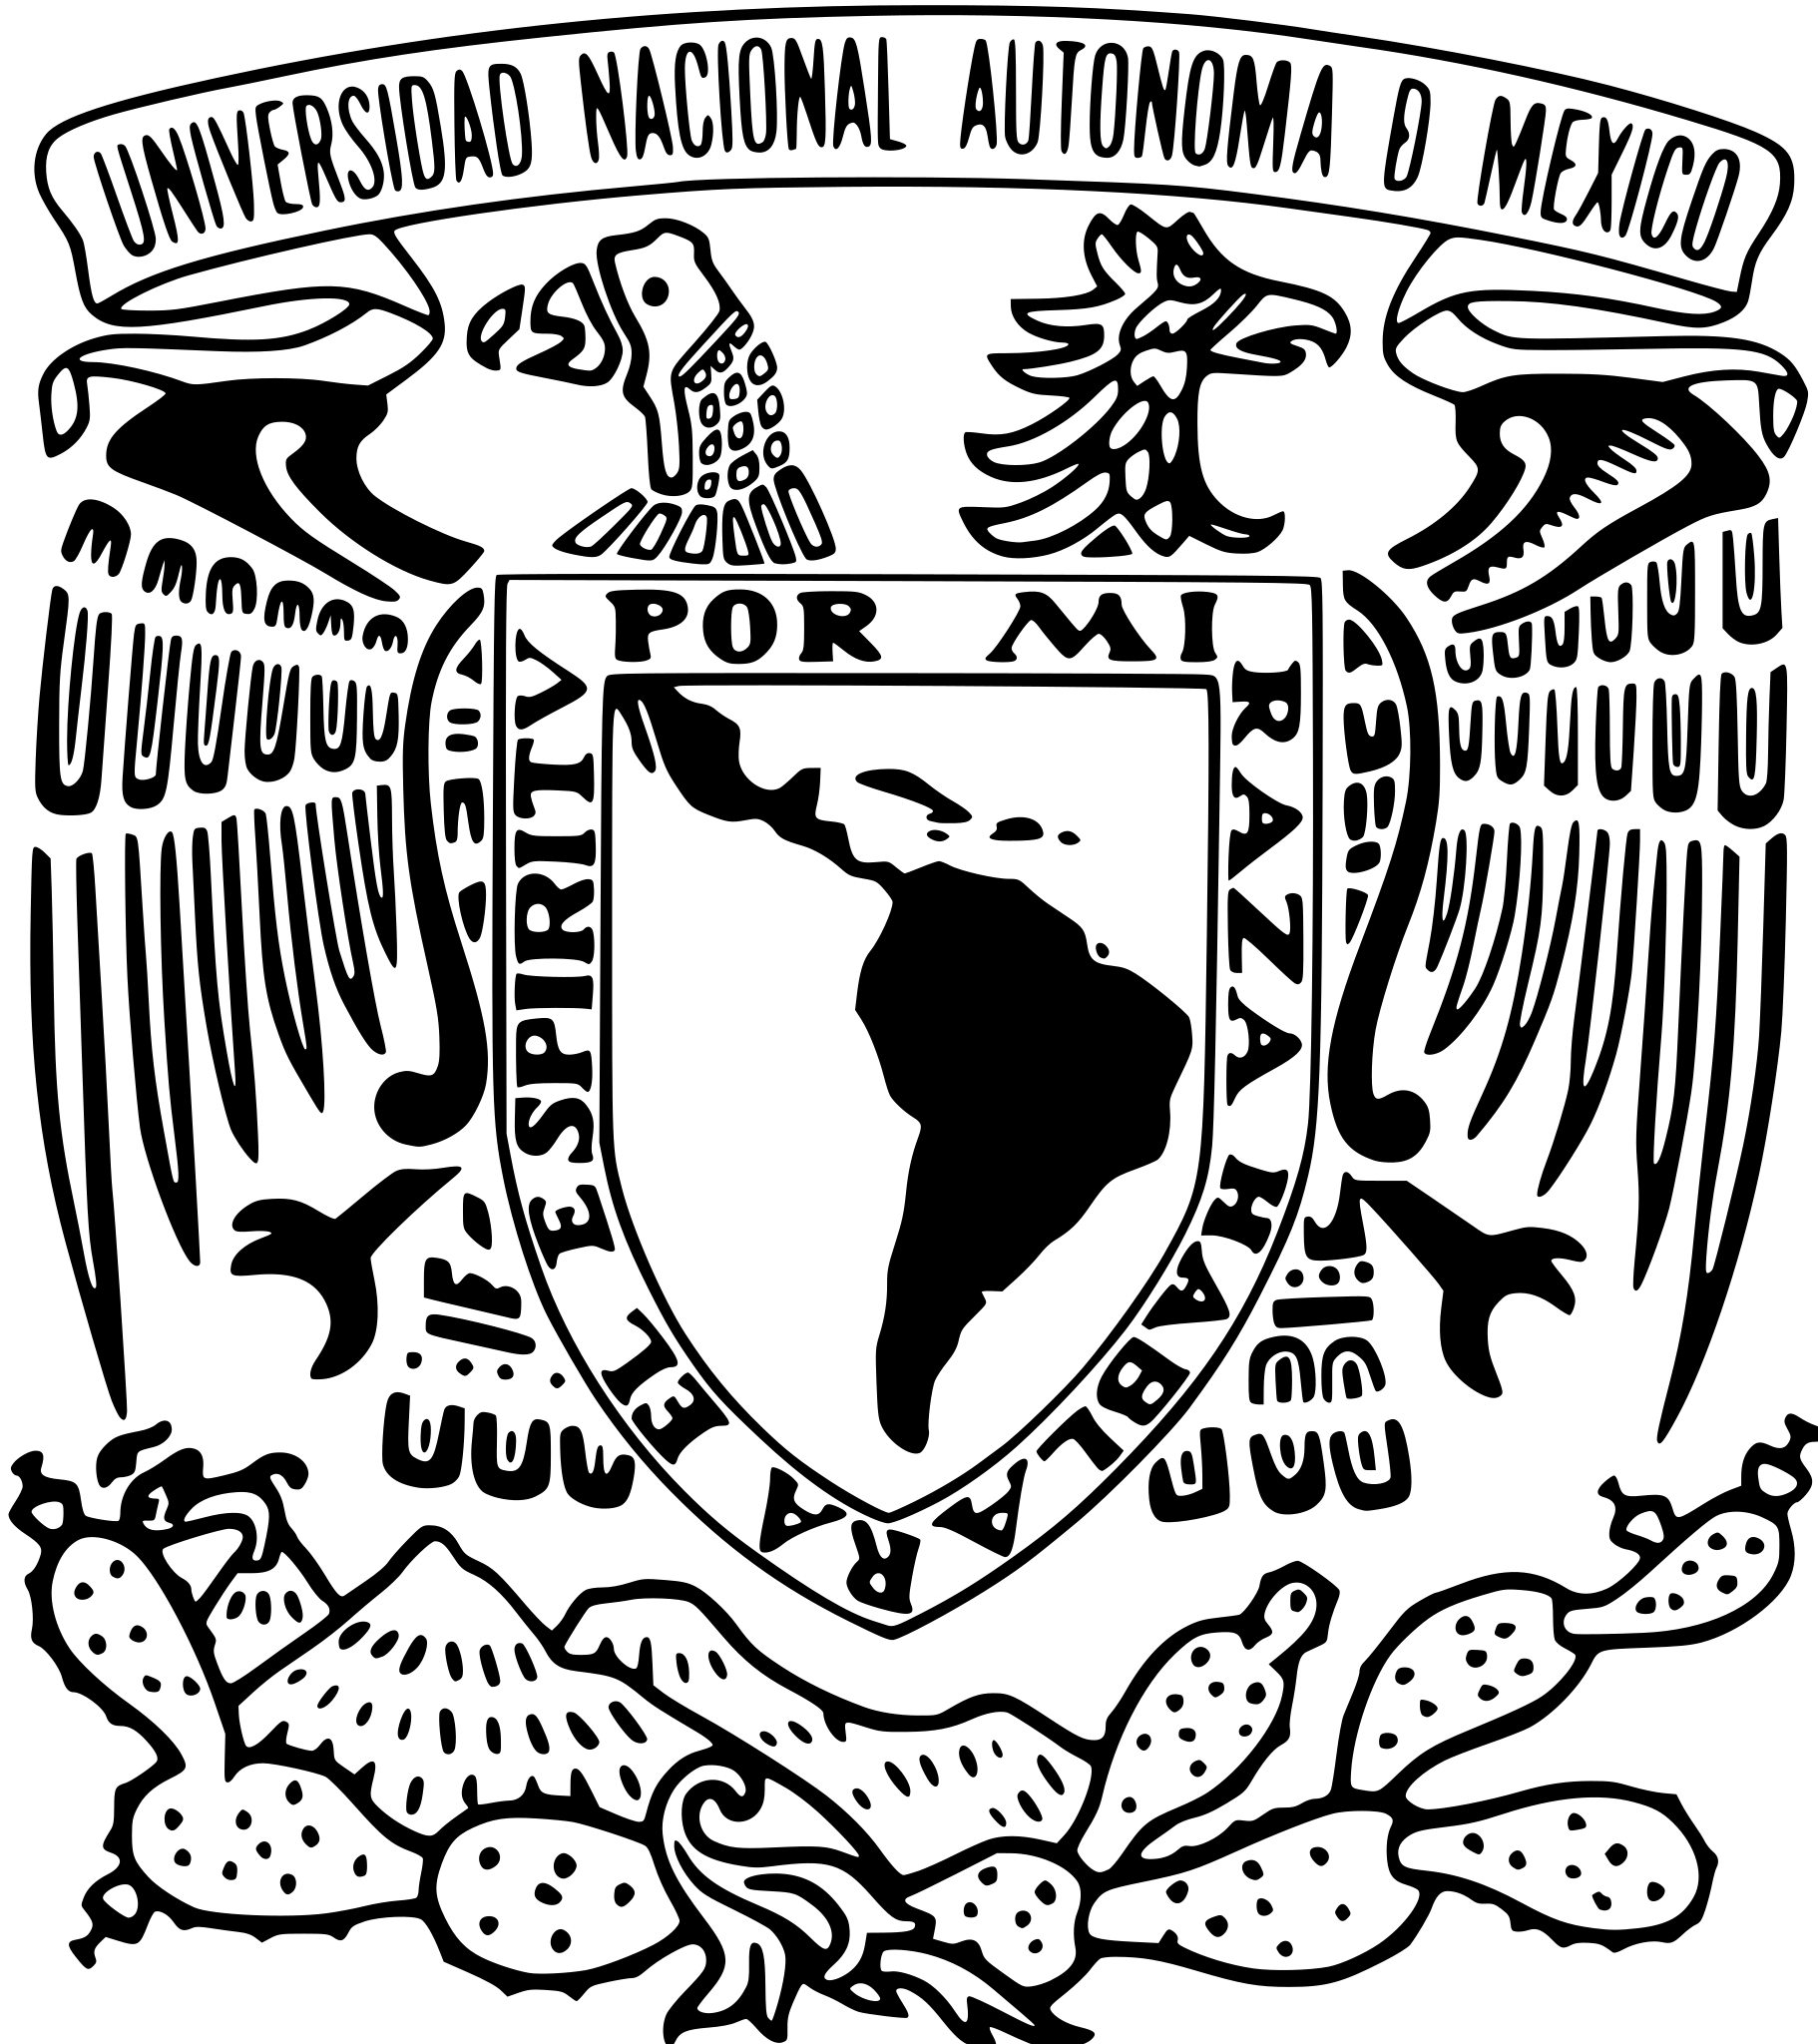
\includegraphics[width=2cm]{EscudoUNAM.png}
\end{minipage}
\hfill
\begin{minipage}{0.4\textwidth}
    \flushright % Alinea la imagen a la derecha dentro de la minipage
    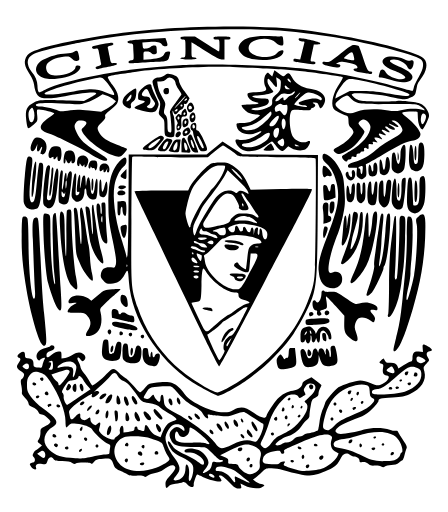
\includegraphics[width=2cm]{EscudoFC.png}
\end{minipage}

%\vspace{0.1cm} % Espacio adicional debajo de las imágenes
%CONFIGURACIÓN DEL ENCABEZADO

\vspace{-2cm}
 
\pagestyle{plain}
\
 
\begin{center}\vspace{-1cm}
\textbf{\large Práctica 1\\ Ley de enfriamiento de Newton}\\   %TITULO
Brown Brittenham Erik, Arcibar Navarrete Hernán, Mendoza Lara José Alfredo\\
\vspace{0.3cm}
\small\textit{Facultad de ciencias, Universidad Nacional Autónoma de México, 27 de agosto del 2024}%NOMBRE
\end{center}
\rule{\linewidth}{0.1mm}

%DESDE AQUÍ SE ESCRIBE TODO EL CONTENIDO
\normalsize

\begin{mdframed}[backgroundcolor=backcolour, linecolor=none, linewidth=0pt]
\begin{abstract}
    \noindent
En esta práctica experimental se estudió el comportamiento del agua al enfriarse desde determinadas temperaturas (90°C, 80°C, 70°C y 60°C) hasta cierta temperatura determinada (temperatura ambiente 22°C, temperatura con hielo 5°). Con el propósito de conocer la relación entre distintos sistemas que son expuestos a un intercambio térmico (agua, el medio ambiente y hielo). \\ El experimento se dividió en dos partes: la primera parte consistió en observar el tiempo de enfriamiento de agua sin otro tipo de interacción más que la del ambiente en el que se encontraba. En la segunda parte se analizó el tiempo de enfriamiento del agua en un calorímetro al cual se le  vertió hielo suficiente para cubrir el recipiente que contenía el agua y poder comparar los tiempos con el primer experimento. \\ No hubo pérdidas significativas de volumen en el experimento. En ambos experimentos se pudo notar en los datos obtenidos la proporcion de enfriamiento respecto a la diferencia de temperaturas, a mayor diferencia de temperatura entre los medios, mas rápido se produjo el intercambio térmico y más se acercaba al equilibrió del sistema, peo conforme la diferencia disminuye se demora más en bajar la temperatura, lo que coincide con los valores teóricos de la Ley de enfriamiento de Newton. Es recomendable al trabajar con el hielo ser meticuloso y rápido con las medidas, pues es un enfriamiento mucho mas acelerado y llega a ser inexacto si no se tiene cuidado.
\end{abstract}
\end{mdframed}
\small\textbf{Palabras clave:} \textit{temperatura, tiempo, enfriamiento, equilibio térmico}
\normalsize

\renewcommand{\abstractname}{Abstract}
\begin{mdframed}[backgroundcolor=backcolour, linecolor=none, linewidth=0pt]
\begin{abstract}
    \noindent
In this experimental practice, the behavior of water when cooled from certain temperatures (90°C, 80°C, 70°C and 60°C) to a certain specific temperature (ambient temperature 22°C, temperature with ice 5°) was studied with The purpose of knowing the relationship between the temperature differences of two media (water, the environment and ice) in the cooling of water. The experiment was divided into two parts: the first part consisted of observing the cooling time of water without any other type of interaction other than the environment. In the second part, the cooling time of the water was analyzed in a calorimeter into which enough ice was poured to cover the container containing the water and to be able to compare the times with the first experiment. There were no significant volume losses in the experiment. In both experiments, it could be noted in the data obtained, the proportion of cooling with respect to the difference in temperatures, the greater the difference in temperature between the media, the faster it cooled, and as it approached thermal equilibrium, it took longer to lower its temperature. . , which coincides with the theoretical values of Newton's Law of Cooling. It is advisable when working with ice to be meticulous and quick with it as it cools much more quickly and becomes inaccurate.
\end{abstract}
\end{mdframed}
\small\textbf{Keywords:} \textit{temperature, time, cooling, exponential}
\normalsize

\begin{multicols}{2}

\section{Introducción}
La ley de enfriamiento de Newton describe el proceso por el cual un cuerpo intercambia calor con su entorno, enfriándose o calentándose dependiendo de la diferencia de temperatura entre el cuerpo y el medio ambiente.

En este trabajo experimental, se explorará y verificará la ley de enfriamiento de Newton mediante la medición de la tasa de enfriamiento del agua en diferentes condiciones ambientales como lo es la temperatura ambiente y un entorno frío con hielo. Se observará cómo la diferencia de temperatura entre el objeto y su entorno influye en la velocidad de pérdida de calor, siguiendo la relación propuesta por Newton. Los resultados obtenidos serán comparados con los valores teóricos previstos, permitiendo evaluar la precisión de la ley en situaciones reales.
El objetivo principal de este experimento es comprender mejor los principios que rigen la transferencia de calor y cómo estos pueden ser aplicados en diversas situaciones prácticas. A través de la recolección y análisis de datos experimentales, se espera demostrar la validez de la ley de enfriamiento de Newton y su relevancia en la predicción del comportamiento térmico de los cuerpos.

\section{Marco teórico}

La Ley de Enfriamiento de Newton es un principio fundamental en la física térmica que describe el proceso de transferencia de calor entre un cuerpo y su entorno. Formulada por Isaac Newton en el siglo XVIII, esta ley establece que la velocidad a la que un cuerpo cambia su temperatura es proporcional a la diferencia de temperatura entre el cuerpo y el medio ambiente. Este concepto es ampliamente utilizado para modelar fenómenos de enfriamiento y calentamiento en diversas aplicaciones científicas y tecnológicas.

La razón de cambio de temperatura de un objeto es proporcional a la diferencia de su temperatura con el ambiente-

\begin{equation}
\frac{dT}{dt} = k(T(t)-T_A)
\end{equation}

\begin{itemize}
    \item $\frac{dT}{dt}$  es la tasa de cambio de la temperatura del cuerpo con respecto al tiempo.
    \item $T$ es la temperatura del cuerpo en un instante de tiempo específico.
    \item $T_A$ es la temperatura del entorno o medio ambiente.
    \item $k$ es una constante de proporcionalidad que depende de las características del cuerpo y del entorno, como la conductividad térmica y las propiedades de la superficie del cuerpo.
\end{itemize}

La ecuación indica que la velocidad a la que la temperatura de un cuerpo cambia con el tiempo es directamente proporcional a la diferencia entre la temperatura del cuerpo y la del entorno. Esto implica que cuanto mayor sea la diferencia de temperatura, más rápida será la transferencia de calor.\\

\textbf{\\Solución}

\begin{equation}
    \frac{dT}{T-T_A} = k dt
\end{equation}

Ahora debemos integrar ambos lados.
\begin{equation}
    \int \frac{dT}{T-T_A} = \int k dt
\end{equation}

Esto nos da como resultado:
\begin{equation}
    \ln |T - T_A| = kt + C
\end{equation}

Tambien podemos considerar cuanto t=0  $T_0$ es
\begin{equation}
    T(t) = T_A + (T-0-T_A) e^{kt}
\end{equation}

Donde C es la constante de integración.\\ Al resolver la ecuación para T se obtiene:
\begin{equation}
    T-T_A = e^{kt+C} =e^{kt} \cdot e^{C} = e^{kt} \cdot C
\end{equation}
\begin{equation}
    T(t) = T_A + Ce^{kt}
\end{equation}
La ecuacion (6) ya es la funcion de temperatura respecto al tiempo.\\

\begin{equation}
    \ln (T(t) - T_A) = kt + \ln (T_0 - T_A)
\end{equation}

\textbf{\\Algunas aplicaciones actuales de la Ley de enfriamiento son:}
\begin{itemize}
    \item Física: Para describir el enfriamiento de cuerpos en diferentes medios.
    \item Ingeniería: En el diseño de sistemas de enfriamiento.
    \item Criminalística: En la estimación del tiempo de muerte en función de la temperatura corporal.
    \item Culinaria: Para modelar cómo los alimentos pierden o ganan calor en diferentes condiciones.
\end{itemize}
%\section{Dispositivo experimental}
%Siempre resultara útil poder escribir el código que uno uso para poder realizar cálculos o gráficos, y si bien, es mucho mejor enviar el código como un archivo a parte, aveces tener una previsualización en el informe basta y sobra. Para esto se tienen dos módulos muy similares, elige el que más te guste para usar.\par
%\end{multicols}
%Es posible imprimir código con el paquete \textbf{lstlistings}:

%\newpage
%También es posible con el paquete \textbf{Minted}:
%\begin{mdframed}[backgroundcolor=backcolour]
  
%\end{mdframed}
%\begin{multicols}{2}

%Cabe destacar que estos paquetes no reconocen tildes, comillas dobles o cualquier carácter fuera del formato UTF-8, por lo que hay que tener cuidado, ya que puede producir errores o directamente no compilar el pdf.

\section{Metodología}
\subsection{Materiales}
Los materiales utilizados para el experimento fueron los siguientes:
\begin{itemize}
    \item Un vaso de precipitados de vidrio de 250 mL.
    \item Una parrilla eléctrica.
    \item Malla de asbesto para colocar el vaso en la parrilla.
    \item Una probeta de plástico para medir el volumen de agua (Incertidumbre de ±5 mL).
    \item Termómetro de alcohol (Incertidumbre de ±0.5 °C).
    \item Cronómeto digital.
    \item Soporte universal.
    \item Pinza de 3 dedos.
    \item Nuez.
    \item Guantes de protección.
    \item Calorímeto.
    \item Hielo.
    \item Tapetes térmicos.
\end{itemize}


\subsection{Procedimiento}
Debido a que el experimento se dividió en dos partes, se tiene que explicar detalladamente cada una de ellas. Es importante mencionar que ambos procedimientos se hicieron a una temperatura ambiental de 21 °C de acuerdo a lo registrado con nuestro termómetro (este dato tiene mayor relevancia en la primera parte que en la segunda).


\textbf{Primera parte}\\
El primer paso fue llenar nuestro vaso de precipitados con 200 mL de agua previamente medidos en la probeta, colocar la malla sobre la parrilla para encenderla y comenzar a calentar el agua.
\\Una vez  montado el sistema para calentar el agua, debimos asegurarnos de monitorear el cambio de temperatura con el termómetro y que el sistema llegase a la temperatura deseada. Esto se hizo con el soporte universal, la nuez y la pinza de tres dedos, en esto sostuvimos el termómetro de manera que pudiéramos observar continuamente el cambio en la temperatura.
\\Se elevó la temperatura del agua a 95 °C para asegurarnos de poder comenzar nuestra medición en los 90 °C ya que debíamos tener en consideración la temperatura que se podía perder al retirar el agua de la parrilla, colocarla en el tapete y volver a incorporar el termómetro para visualizar la temperatura. 
\\Efectivamente este paso se realizó como ya se detalló previamente y comenzamos nuestra medición con el termómetro juesto en los 90 °C, así continuamos con mediciones cada ciertos intervalos hasta llegar a 45 °C, esta temperatura fue elegida por consenso en el laboratorio para optimizar el tiempo de realización del experimento.
\\Este procedimiento se repitió con las demás temperaturas de 80 °C, 70 °C y 60 °C.


\begin{figure}[H]
    \centering
    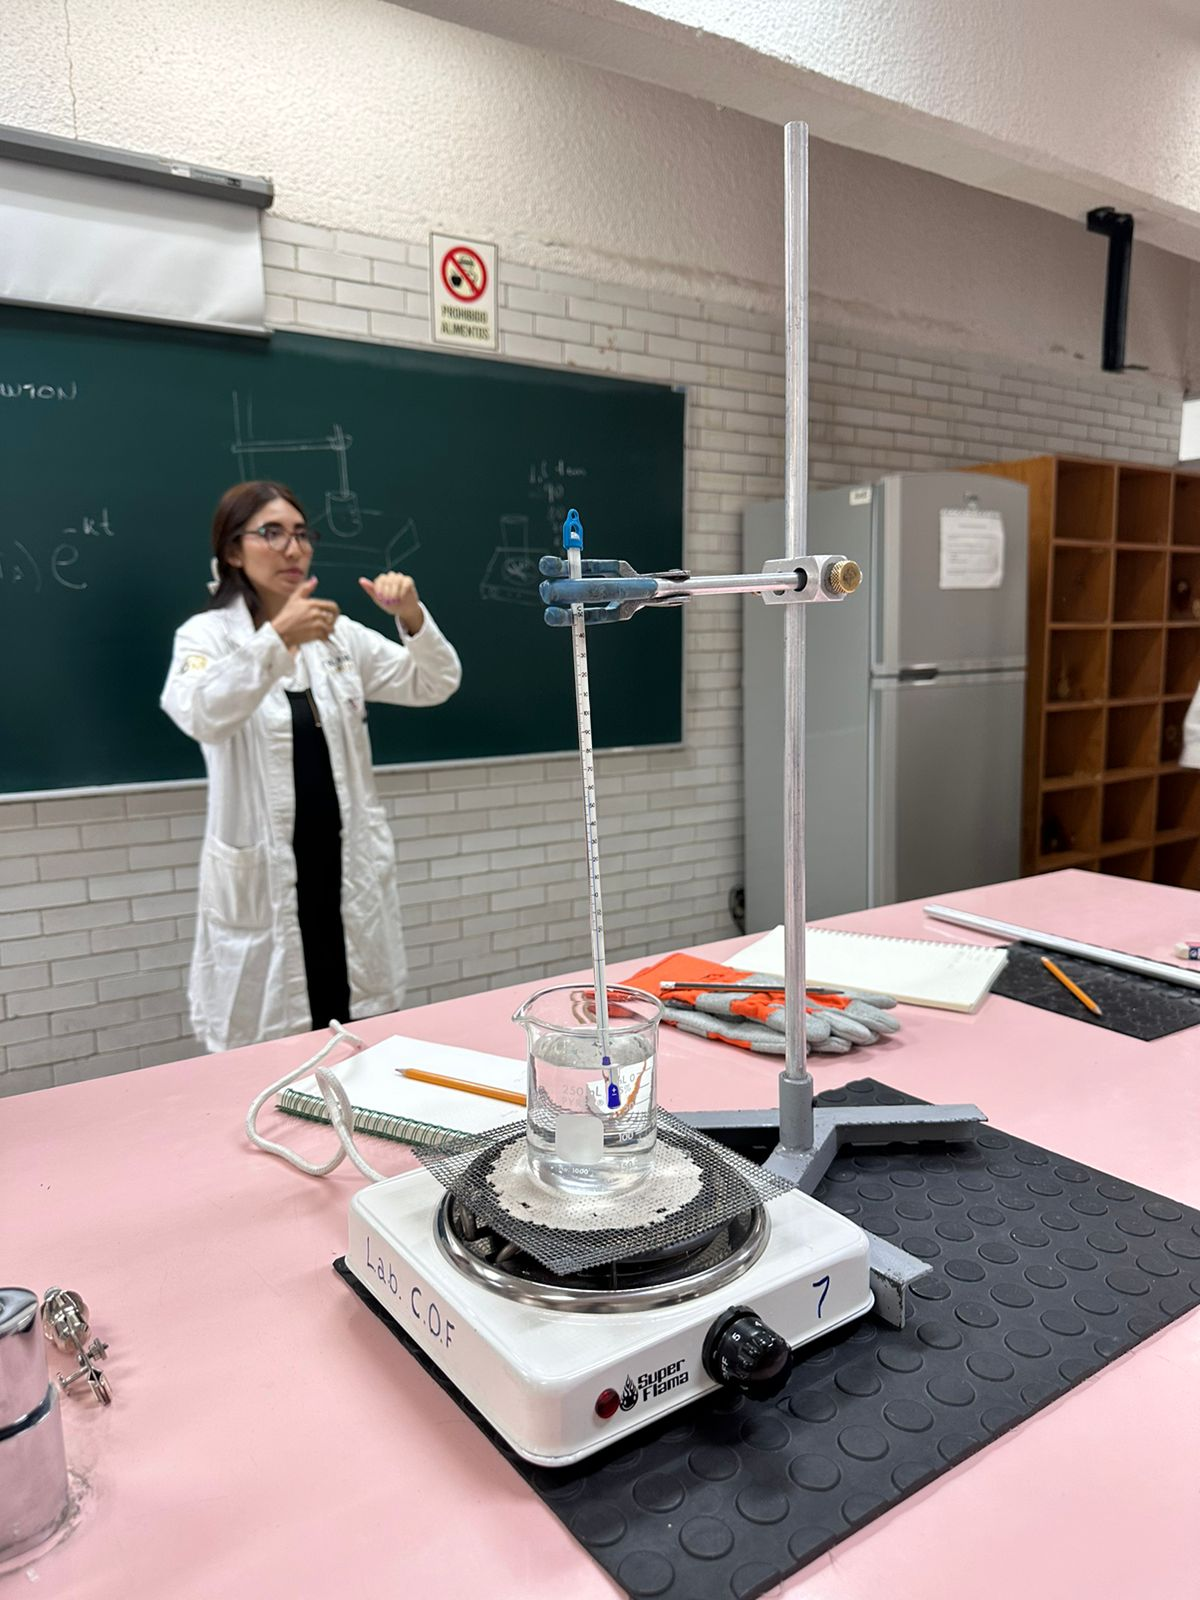
\includegraphics[width=0.7\linewidth]{base.png}
    \caption{Equipo de laboratorio montado}
    \label{fig:enter-label}
\end{figure}



\textbf{Segunda parte}
\\Para la segunda parte se procedió a triturar algunos cubos de hielo para colocarlos en el calorímetro, tanto en la base como en las paredes del mismo, el resto de este procedimiento fue análogo al de la primera parte, pero con una diferencia importante: el agua esta vez no fue enfriada solo con el intercambio térmico que se produce con el contacto con el ambiente, sino que la vertimos en el calorímetro que rellenamos con hielo y de esta manera pudimos empezar a tomar nuestras medidas correspondientes. Inmediatamente fue notorio que por la mayor diferencia de temperatura entre los sistemas la temperatura empezó a bajar mucho más rápido, pero esto lo analizaremos mejor en nuestra discusión de resultados.\\
Este procedimiento se repitió con las demás temperaturas de 80 °C, 70 °C y 60 °C. En esta sección la temperatura final en todos los casos fue de 5 °C.

\begin{figure}[H]
    \centering
    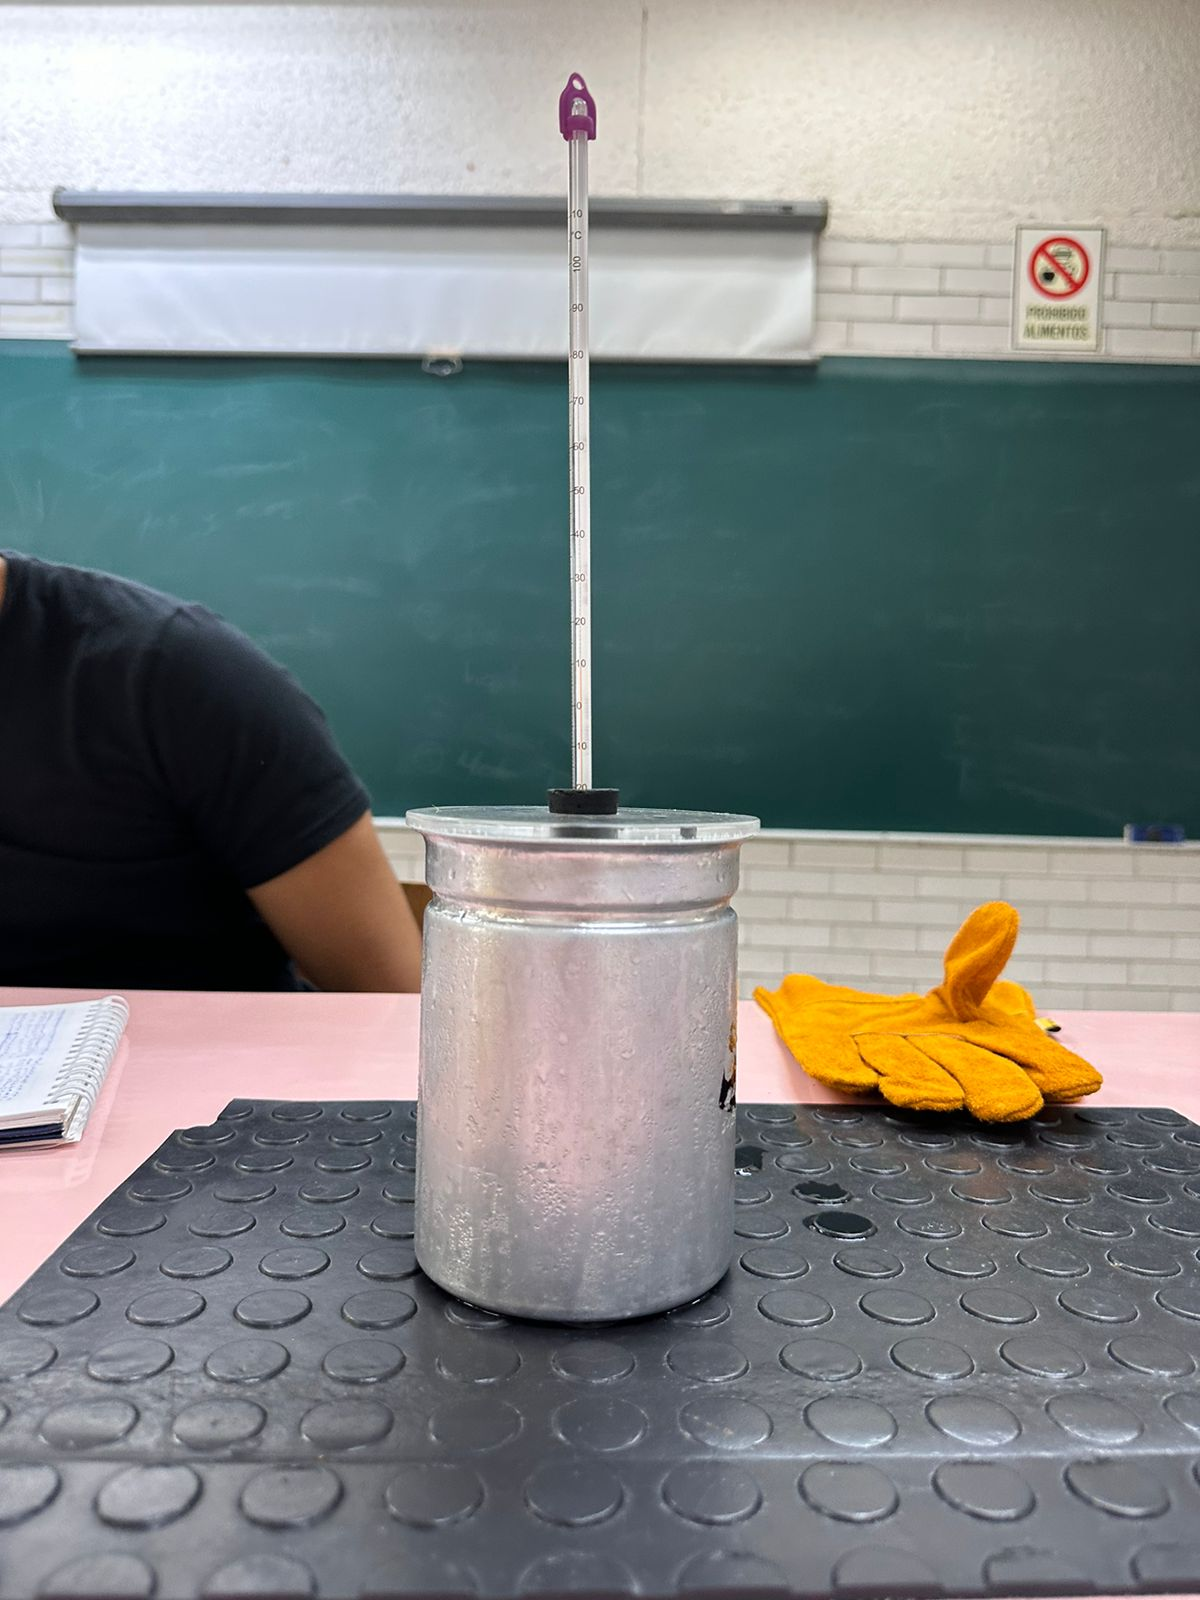
\includegraphics[width=0.7\linewidth]{calor.png}
    \caption{Calorímetro con termómetro montado}
    \label{fig:enter-label}
\end{figure}

\section{Resultados}

Las condiciones en las que se trabajó en el laboratorio para todos los experimentos fue la misma con una temperatura ambiente constante de 21 °C $\pm$   0.5 °C. \\
Ya que el experimento está dividido en dos partes, analizaremos los resultados también en dos secciones.

\subsection{Intercambio térmico a temperatura ambiente}
Primeramente, en la tabla 1 presentamos los tiempos generales de enfriamiento que se presentaron para cada temperatura hasta alcanzar 45 °C.


\begin{tabular}{|c|c|c|}
    \hline
    $T_0$ $\pm$   0.5 (°C) & Tiempo (s) & T. final $\pm$   0.5 (°C)\\ \hline
    90° & 2100 &  45 \\ \hline
    80° & 1740  & 45 \\ \hline
    70° & 1500 & 45 \\ \hline
    60° & 1080 & 45 \\ \hline
\end{tabular}

Tabla 1. Tiempos totales de enfriamiento hasta 45°C

 Enseguida tenemos los datos de cómo se describe el decremento de temperatura con respecto al tiempo, esto nos deja ver una clara proporcionalidad entre el tiempo y la temperatura; observemos cómo mientras más se acerca a la temperatura final, los intervalos de tiempo se hacen mas grandes.

\begin{tabular}{|c|c|}
	\hline
	\textbf{Tiempo (s)} & \textbf{Temperatura } $\pm$ 0.5 $^\circ$C \\ \hline
		0    & 90.0  \\ \hline
		30   & 88.0  \\ \hline
		60   & 86.0  \\ \hline
		90   & 84.0  \\ \hline
		120  & 83.0  \\ \hline
		150  & 81.5  \\ \hline
		180  & 80.0  \\ \hline
		210  & 78.5  \\ \hline
		240  & 77.5  \\ \hline
		270  & 76.0  \\ \hline
		300  & 75.0  \\ \hline
		360  & 73.0  \\ \hline
		420  & 70.0  \\ \hline
		480  & 69.0  \\ \hline
		540  & 67.0  \\ \hline
		600  & 65.0  \\ \hline
		660  & 64.0  \\ \hline
		720  & 63.0  \\ \hline
		780  & 62.0  \\ \hline
		840  & 61.0  \\ \hline
		900  & 60.0  \\ \hline
		1020 & 57.0  \\ \hline
		1140 & 55.0  \\ \hline
		1260 & 54.0  \\ \hline
		1380 & 52.0  \\ \hline
		1500 & 51.0  \\ \hline
		1620 & 50.0  \\ \hline
		1740 & 48.0  \\ \hline
		1860 & 47.0  \\ \hline
		1980 & 46.0  \\ \hline
		2100 & 45.0  \\ \hline
\end{tabular}
\\Tabla 2. Mediciones de la temperatura con respecto a intervalos de tiempo para 90°C.
    

La Tabla 3 igualmente nos muestra los datos del tiempo en todo su proceso de enfriamiento donde podemos apreciar como existe una diferencia de tiempo con respecto a los 90° a pesar de no ser una diferencia de temperatura tan grande. Esto es una interesante observación pues nos describe como se comporta el enfriamiento con distintas temperaturas.

Si bien la diferencia en los tiempos finales parece muy grande, debemos considerar que el liquido a 80° solo se midió su temperatura hasta que disminuyó a 47°C, un error de medición que afecta el tiempo final, pero si tomamos en cuenta los 47°C de la tabla 2 podemos ver como sigue existiendo una diferencia de tiempo porlo que no perdemos generalidad a pesar de esa medición equivocada.

Esto a su vez, nos deja ver como la temperatura inicial no afecta en la proporcionalidad de su enfriamiento, solamente en el tiempo final, pues si miramos (por ejemplo) la temperatura de 57° para ambas tablas vemos que ambas disminuyen 2 grados en dos minutos.\\ Lo que nos dice que la temperatura decrece siempre de manera consistente de acuerdo a la Ley de enfriamiento de Newton, es decir, que la temperatura disminuirá de la misma manera en los mismos intervalos de tiempo aunque sus temperaturas iniciales hayan sido distintas.\\



Tabla 3. Mediciones de la temperatura con respecto a intervalos de tiempo 80°C.

\begin{tabular}{|c|c|}
	\hline
	\textbf{Tiempo (s)} & \textbf{Temperatura  $\pm$ 0.5 $^\circ$C} \\ \hline
	0    & 80  \\ \hline
	30   & 79  \\ \hline
	60   & 77  \\ \hline
	90   & 75  \\ \hline
	120  & 74  \\ \hline
	150  & 73  \\ \hline
	180  & 72  \\ \hline
	210  & 70  \\ \hline
	270  & 69  \\ \hline
	330  & 67  \\ \hline
	390  & 65  \\ \hline
	450  & 64  \\ \hline
	510  & 63  \\ \hline
	570  & 61  \\ \hline
	690  & 59  \\ \hline
	810  & 57  \\ \hline
	930  & 55  \\ \hline
	1050 & 54  \\ \hline
	1170 & 52  \\ \hline
	1350 & 50  \\ \hline
	1530 & 48  \\ \hline
	1710 & 47  \\ \hline
\end{tabular}


Tabla 4. Mediciones de la temperatura con respecto a intervalos de tiempo 60°C.\\

\begin{tabular}{|c|c|}
	\hline
	\textbf{Tiempo (s)} & \textbf{Temperatura  $\pm$ 0.5 $^\circ$C}  \\ \hline
	0    & 60  \\ \hline
	30   & 59  \\ \hline
	60   & 58  \\ \hline
	90   & 57  \\ \hline
	120  & 56  \\ \hline
	150  & 55  \\ \hline
	180  & 54  \\ \hline
	210  & 53  \\ \hline
	240  & 52  \\ \hline
	270  & 51  \\ \hline
	300  & 50  \\ \hline
	330  & 50  \\ \hline
	360  & 49  \\ \hline
	390  & 48  \\ \hline
	420  & 48  \\ \hline
	450  & 47  \\ \hline
	480  & 46  \\ \hline
	510  & 46  \\ \hline
\end{tabular}
\end{multicols}

\begin{multicols}{2}
Tabla 5. Mediciones de la temperatura con respecto a intervalos de tiempo 70°C.

\begin{tabular}{|c|c|}
	\hline
	\textbf{Tiempo (s)} & \textbf{Temperatura  $\pm$ 0.5 $^\circ$C}  \\ \hline
	0    & 70.0  \\ \hline
	30   & 69.0  \\ \hline
	60   & 68.0  \\ \hline
	90   & 67.0  \\ \hline
	120  & 66.5  \\ \hline
	150  & 66.0  \\ \hline
	180  & 65.0  \\ \hline
	210  & 64.5  \\ \hline
	240  & 63.0  \\ \hline
	270  & 62.5  \\ \hline
	300  & 62.0  \\ \hline
	360  & 60.0  \\ \hline
	420  & 59.0  \\ \hline
	480  & 58.0  \\ \hline
	540  & 57.0  \\ \hline
	600  & 56.0  \\ \hline
	660  & 55.0  \\ \hline
	720  & 54.0  \\ \hline
	780  & 53.0  \\ \hline
	840  & 52.0  \\ \hline
	900  & 51.5  \\ \hline
	1020 & 50.0  \\ \hline
	1140 & 48.5  \\ \hline
	1260 & 47.0  \\ \hline
	1380 & 46.0  \\ \hline
	1500 & 45.0  \\ \hline
\end{tabular}


En la Tabla 4 y Tabla 5 tambien podemos observar como el tiempo final es menor, esto se debe a las temperaturas iniciales, que causan una diferencia al empezar desde una temperatura menor.

Analizando los datos de las tablas podemos observar como los intervalos de tiempo para que disminuya la temperatura van creciendo conforme se acercan a la temperatura final (o entre mas tiempo pase) por lo que ya podemos darnos una idea de omo podría ser la gráfica, asemejandose a una funcion asintótica. Lo que nos revela como entre mayor sea la diferencia de temperaturas entre la temperatura ambiente y la temperatura del agua, mayor será la rapidez con la que disminuye la temperatura.

Ahora graficaremos las funciones con los datos proporcionados.

Las imagenes fueron graficadas en Rstudio y toman en cuenta todos los datos de las tablas y debido a la extensión de la cantidad de datos, son gráficas bastante detalladas.
\end{multicols}

\begin{figure}[h]
    \centering
    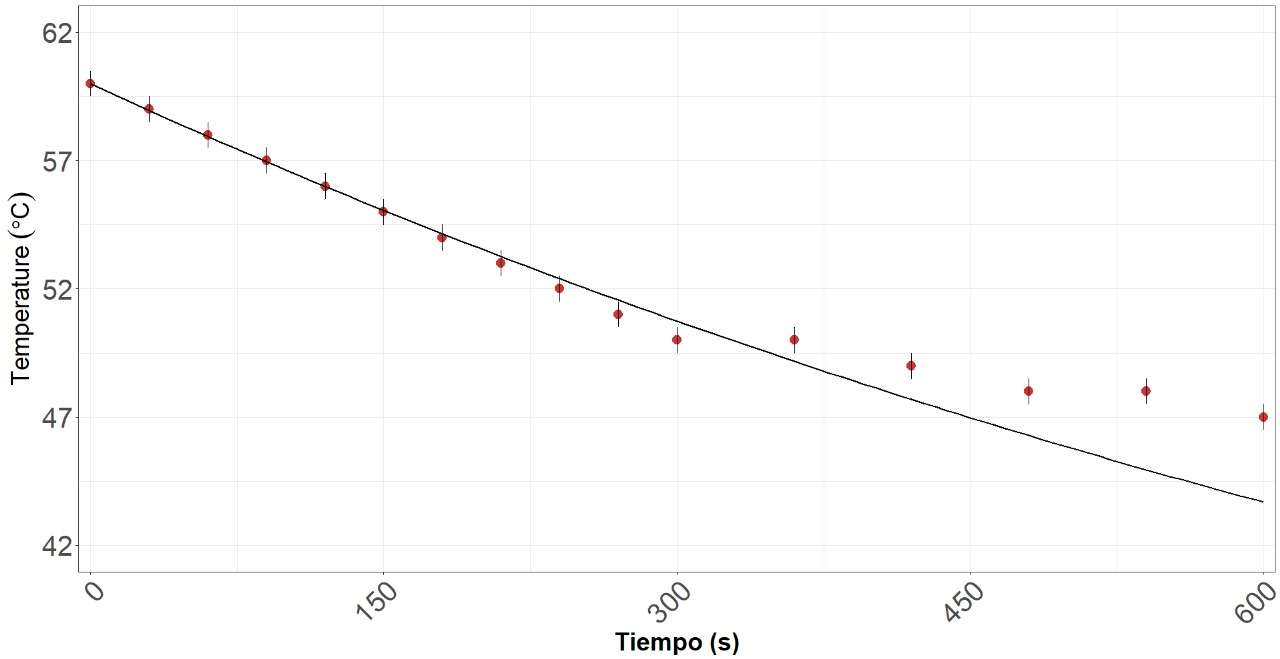
\includegraphics[width=0.9\linewidth]{60.png}
    \caption{Gráfica de la disminución de temperatura desde 60°C}
    \label{fig:enter-label}
\end{figure}

\begin{figure}[h]
    \centering
    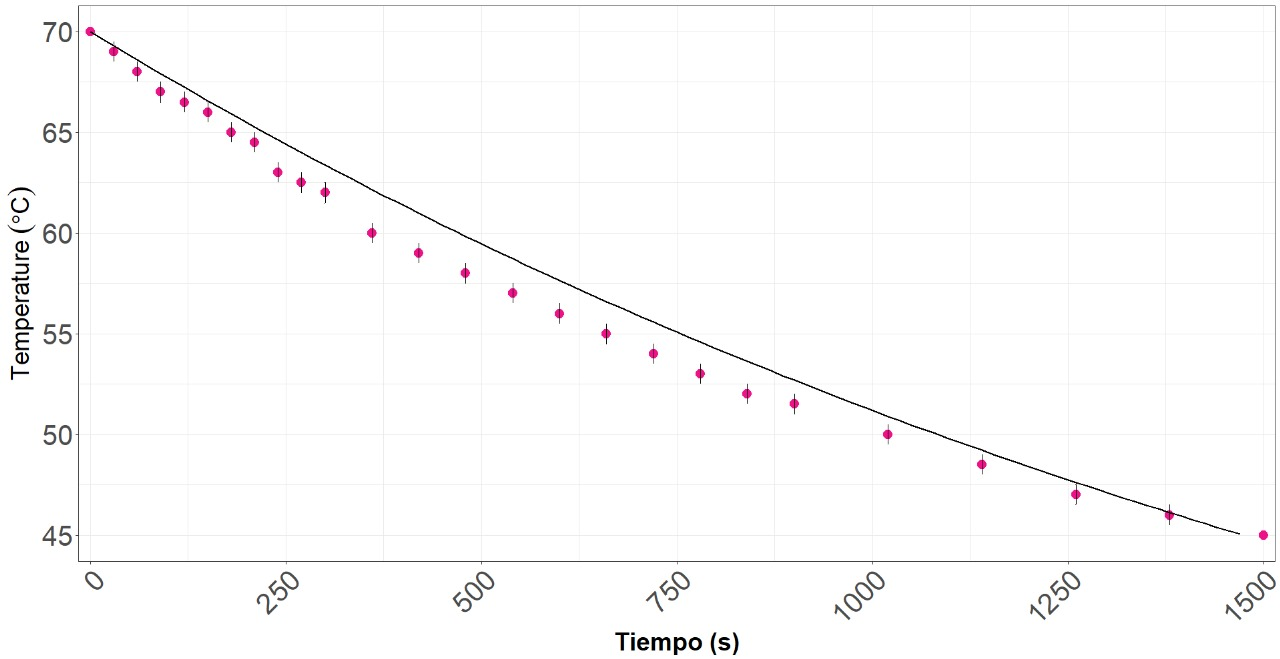
\includegraphics[width=0.8\linewidth]{70.png}
    \caption{Gráfica de la disminución de temperatura desde 70°C}
    \label{fig:enter-label}
\end{figure}
\vspace{0.2cm}

\begin{multicols}{2}
    

Cada gráfica nos dice como la temperatura de un cuerpo cambia a lo largo del tiempo mientras se enfría en un entorno a una temperatura constante. La representación gráfica típica de esta ley es una curva exponencial decreciente. 

Las gráficas linealizadas de la Ley de Enfriamiento de Newton se obtienen al transformar la ecuación exponencial en una forma lineal, lo que facilita la interpretación y el análisis de los datos experimentales. Para obtener una gráfica linealizada, se realiza un cambio de variables que convierte la ecuación exponencial en una ecuación lineal.

\end{multicols}
\begin{figure}[h]
    \centering
    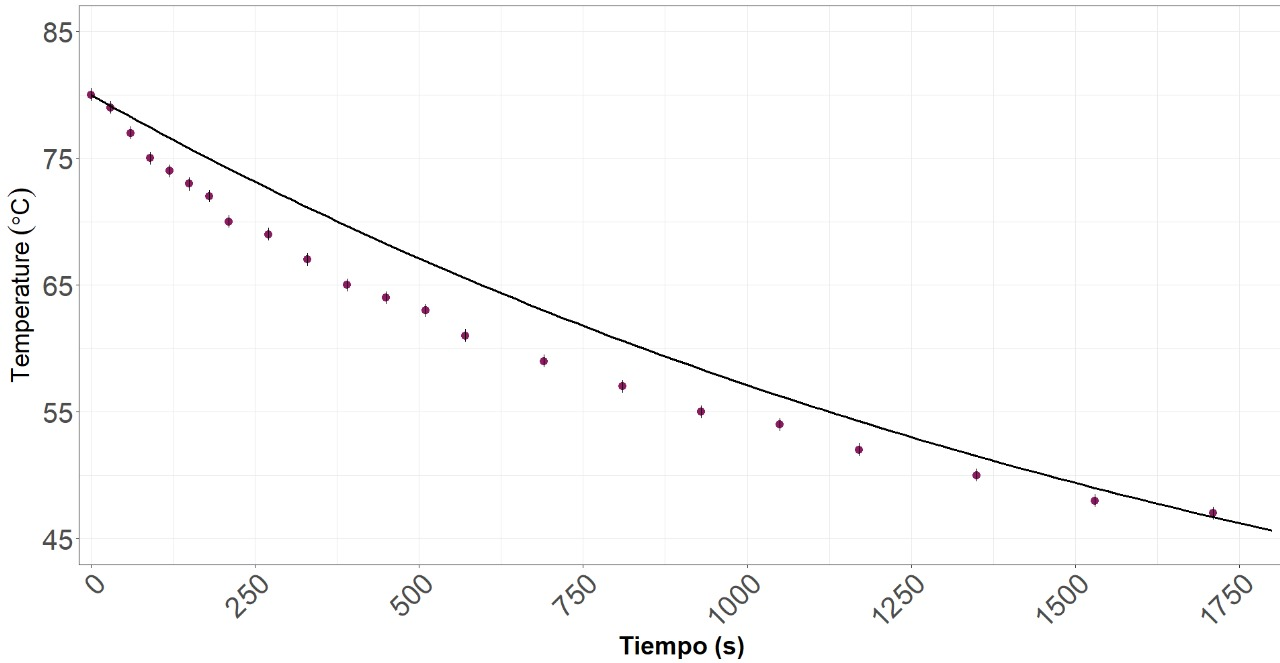
\includegraphics[width=0.9\linewidth]{80.png}
    \caption{Gráfica de la disminución de temperatura desde 80°C}
    \label{fig:enter-label}
\end{figure}

\newpage

\begin{multicols}{2}
    
Estas gráficas representan los datos tiempo-temperatura tal cual fueron tomados, pero ahora se require la observación de las gráficas linealizadas. Las gráficas linealizadas de la Ley de Enfriamiento de Newton se obtienen al transformar la ecuación exponencial en una forma lineal, lo que facilita la interpretación y el análisis de los datos experimentales. Para obtener una gráfica linealizada, se realiza un cambio de variables que convierte la ecuación exponencial en una ecuación lineal.
\end{multicols}
\begin{figure}[h]
    \centering
    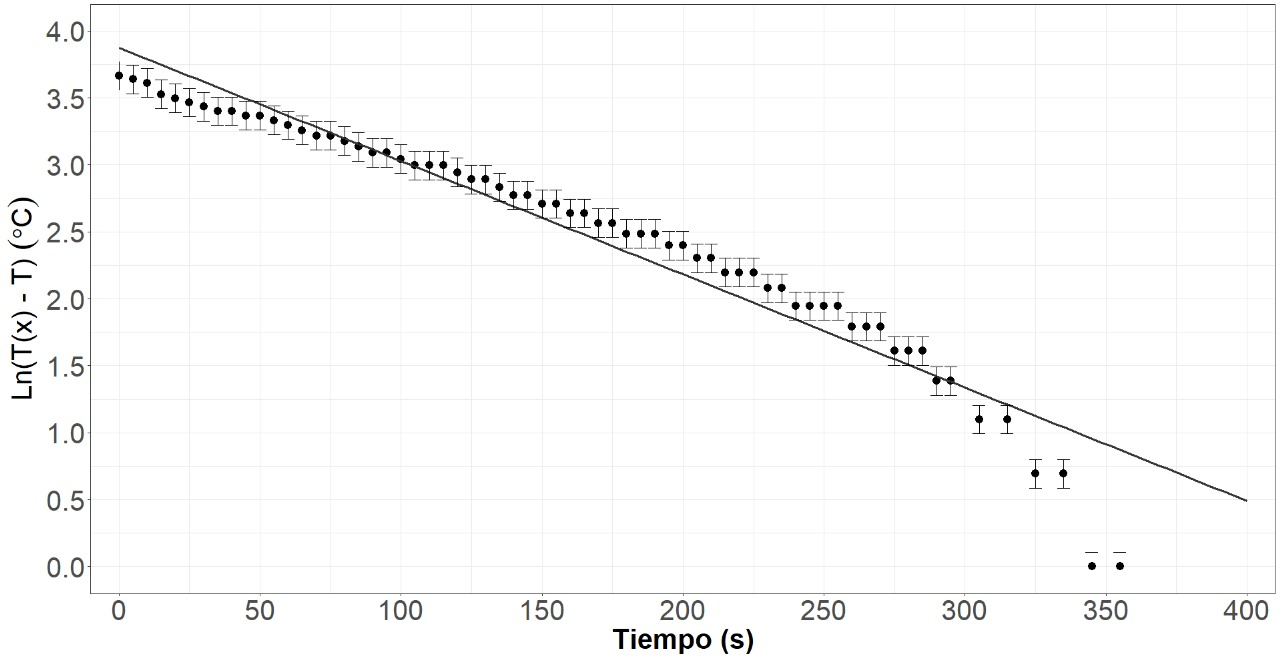
\includegraphics[width=0.8\linewidth]{60lin.png}
    \caption{Gráfica linealizada de la disminución de temperatura desde 60°C}
    \label{fig:enter-label}
\end{figure}

\begin{multicols}{2}
La gráfica linealizada de la Ley de Enfriamiento de Newton proporciona una herramienta útil para analizar datos experimentales, determinar la constante de enfriamiento y verificar la validez del modelo de enfriamiento exponencial. Aqui se muestran las demás gráficas ya linealizadas de los demás experimentos
\end{multicols}
\begin{figure}[h]
    \centering
    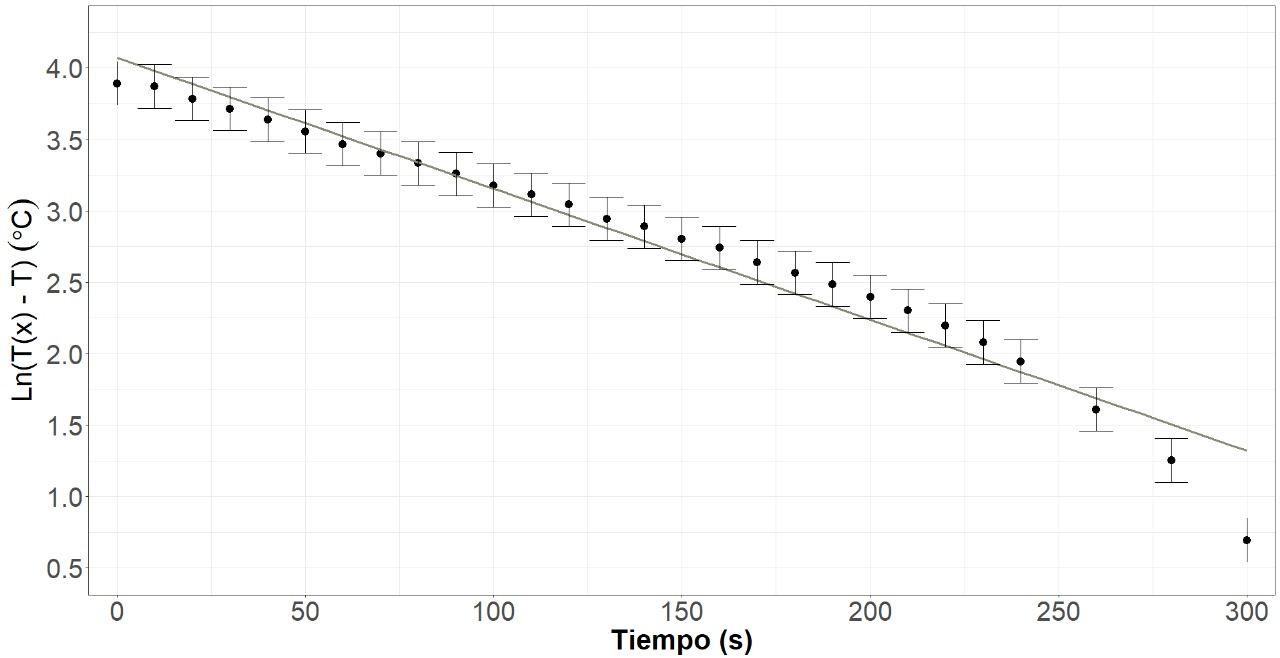
\includegraphics[width=0.8\linewidth]{70lin.png}
    \caption{Gráfica linealizada de la disminución de temperatura desde 70°C}
    \label{fig:enter-label}
\end{figure}
\vspace{2cm}

\begin{figure}[h]
    \centering
    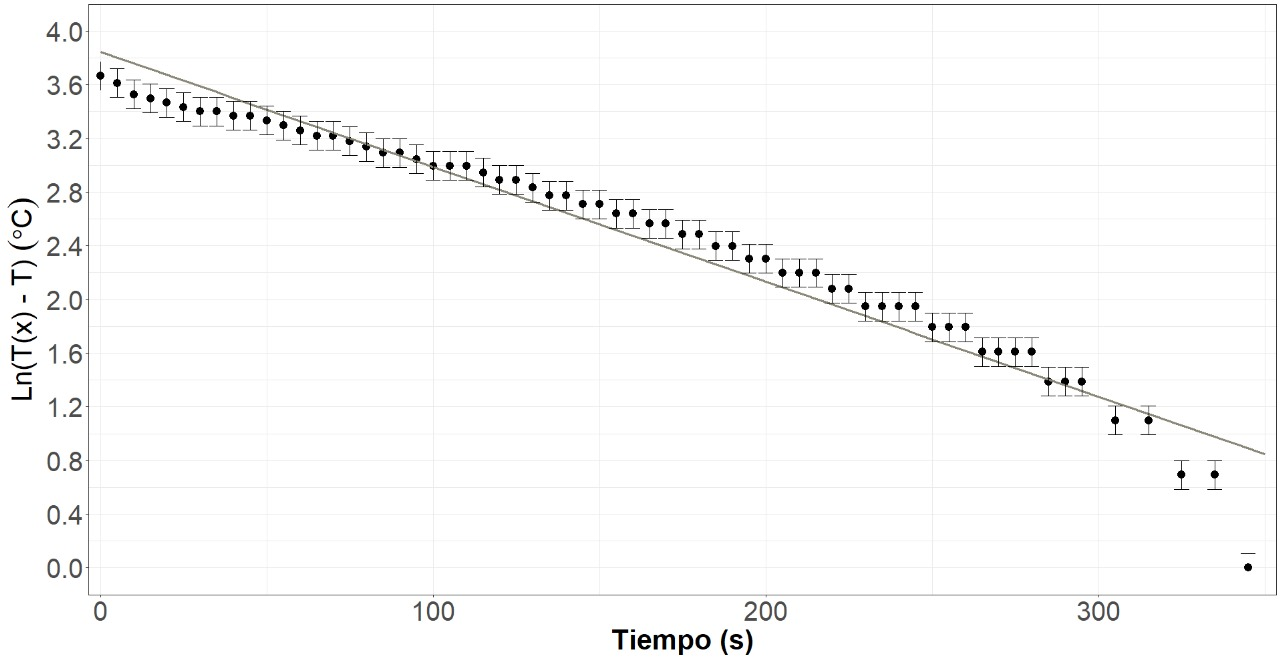
\includegraphics[width=0.8\linewidth]{80lin.png}
    \caption{Gráfica linealizada de la disminución de temperatura desde 80°C}
    \label{fig:enter-label}
\end{figure}

\begin{figure}[H]
    \centering
    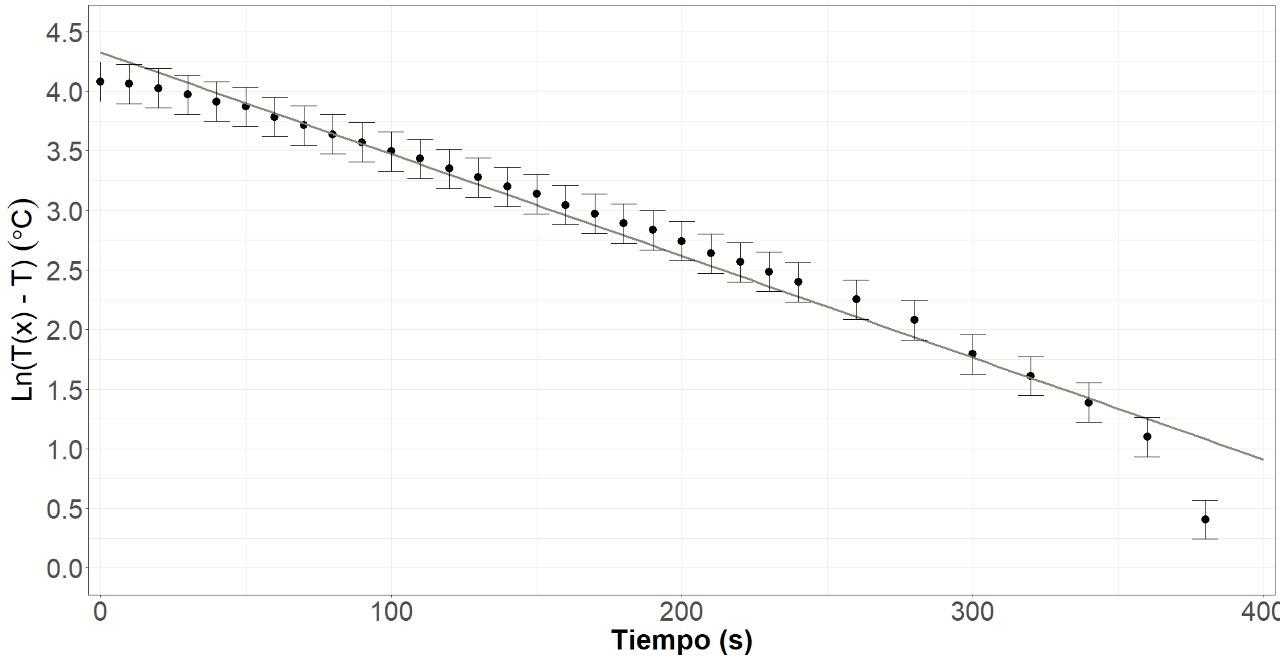
\includegraphics[width=0.8\linewidth]{90lin.png}
    \caption{Gráfica linealizada de la disminución de temperatura desde 90°C}
    \label{Gráfica linealizada de la disminución de temperatura desde 90°C}
\end{figure}
\begin{multicols}{2}
Ahora analicemos brevemente las gráficas del calorímetro puesto que el principio es el mismo, podremos saber igualmente que es lo que ocurres, con la diferencia de que aquí la diferencia entre el líquido y la temperatura del medio se vuelve muy grande lo que va a causar una perdida de temperatura inmediata y muy rapida. El hielo hace que la temperatura mínima que se pueda alcanzar sea mucho menor y la rapidez del enfriamiento tambien lo sea mucho mas, al menos al principio del enfriamiento pues cuando se acerca a la temperatura mínima tambien vuelve a disminuir la velocidad.
\end{multicols}
\begin{center}
\begin{figure}[H]
    \centering
    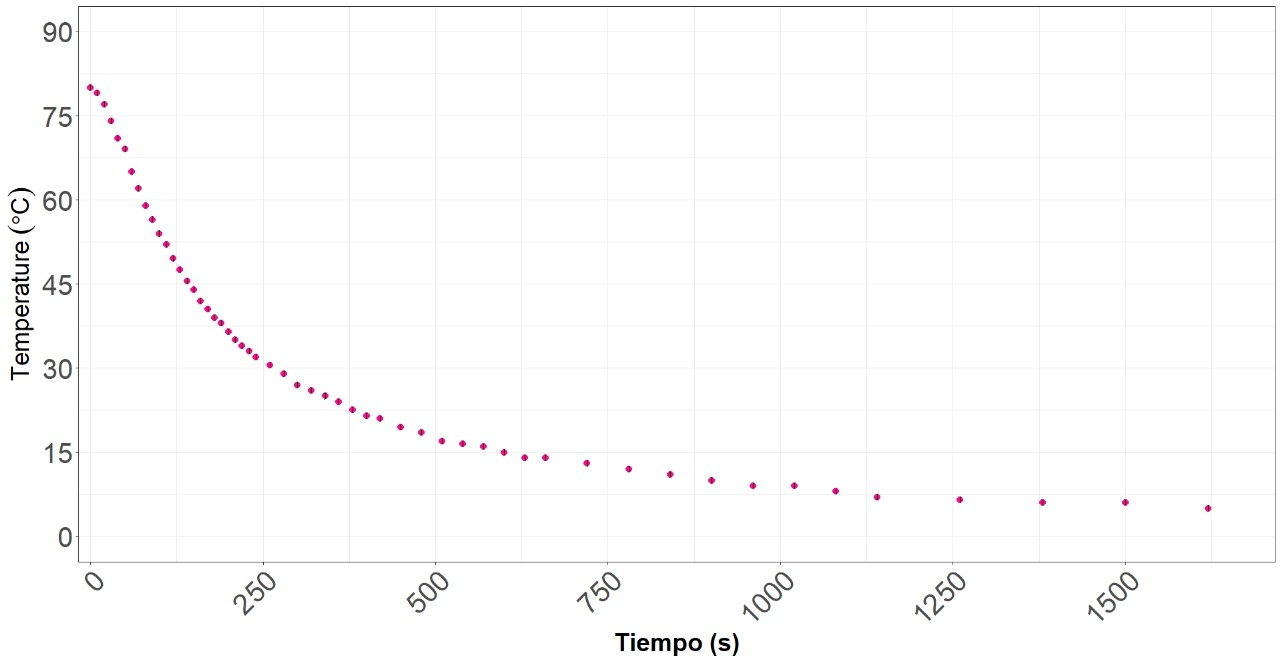
\includegraphics[width=0.8\linewidth]{90cal.png}
    \caption{Gráfica de la disminución de temperatura desde 90°C}
    \label{fig:enter-label}
\end{figure}
\end{center}


\newpage


\begin{multicols}{2}
	\begin{tabular}{|c|c|}
		\hline
		\textbf{Tiempo (s)} & \textbf{Temperatura (°C)} \\ \hline
		0    & 80.0  \\ \hline
		10   & 79.0  \\ \hline
		20   & 77.0  \\ \hline
		30   & 74.0  \\ \hline
		40   & 71.0  \\ \hline
		50   & 69.0  \\ \hline
		60   & 65.0  \\ \hline
		70   & 62.0  \\ \hline
		80   & 59.0  \\ \hline
		90   & 56.5  \\ \hline
		100  & 54.0  \\ \hline
		110  & 52.0  \\ \hline
		120  & 49.5  \\ \hline
		130  & 47.5  \\ \hline
		140  & 45.5  \\ \hline
		150  & 44.0  \\ \hline
		160  & 42.0  \\ \hline
		170  & 40.5  \\ \hline
		180  & 39.0  \\ \hline
		190  & 38.0  \\ \hline
		200  & 36.5  \\ \hline
		210  & 35.0  \\ \hline
		220  & 34.0  \\ \hline
		230  & 33.0  \\ \hline
		240  & 32.0  \\ \hline
		260  & 30.5  \\ \hline
		280  & 29.0  \\ \hline
		300  & 27.0  \\ \hline
		320  & 26.0  \\ \hline
		340  & 25.0  \\ \hline
		360  & 24.0  \\ \hline
		380  & 22.5  \\ \hline
		400  & 21.5  \\ \hline
		420  & 21.0  \\ \hline
		450  & 19.5  \\ \hline
		480  & 18.5  \\ \hline
		510  & 17.0  \\ \hline
		540  & 16.5  \\ \hline
		570  & 16.0  \\ \hline
		600  & 15.0  \\ \hline
		630  & 14.0  \\ \hline
		660  & 14.0  \\ \hline
		720  & 13.0  \\ \hline
		780  & 12.0  \\ \hline
		840  & 11.0  \\ \hline
  \end{tabular}

\begin{tabular}{|c|c|}
		\hline
		\textbf{Tiempo (s)} & \textbf{Temperatura (°C)} \\ \hline
        900  & 10.0  \\ \hline
		960  & 9.0   \\ \hline
		1020 & 9.0   \\ \hline
		1080 & 8.0   \\ \hline
		1140 & 7.0   \\ \hline
		1260 & 6.5   \\ \hline
		1380 & 6.0   \\ \hline
		1500 & 6.0   \\ \hline
		1620 & 5.0   \\ \hline
	
\end{tabular}
  
Tabla 6. Mediciones de la temperatura con respecto a intervalos de tiempo 80°C con el calorímetro.


En la Tabla 6 se ve claramente la Ley de enfriamiento de Newton, al momento de iniciar la medición la perdidad de temperatura durante los primeros segundos fue muy grande y rapida, lo que vuelve a confirmar que a mayor diferencia de temperatura la tasa de pérdida de calor se vuelve mucho mas grande.

Si comparamos los datos con la Tabla 3podemos ver como la diferencia en la la tasa de pérdida de calor es muy distinta, además de que el tiempo final que necesitaron para alcanzar sus temperaturas mínimas difiere mucho.

En la gráfica se puede ver una curva mucho mas pronunciada debido a que la diferencia de temperatura entre los dos medios es mucho mas grande que los experimentos anteriores donde no se usó el calorimetro.

\begin{figure}[H]
    \centering
    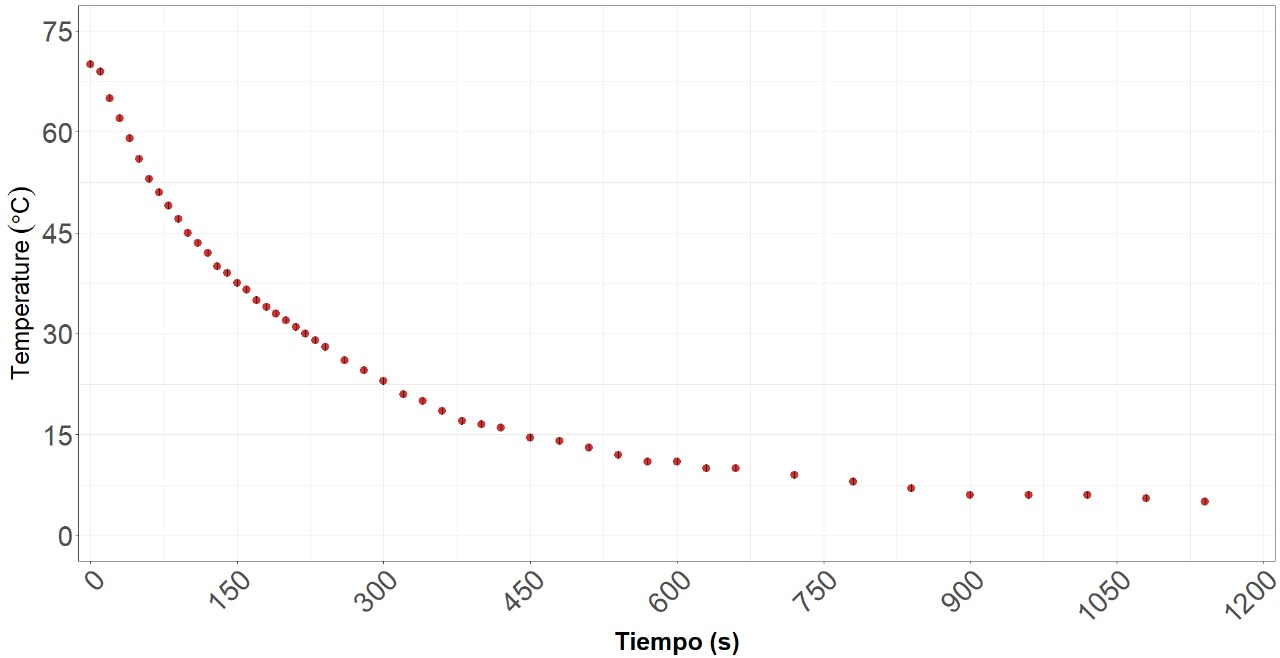
\includegraphics[width=1.2\linewidth]{imagen_2024-08-29_025308306.png}
    \caption{Caption}
    \label{fig:enter-label}
\end{figure}

\newpage
\end{multicols}

\begin{figure}
    \centering
    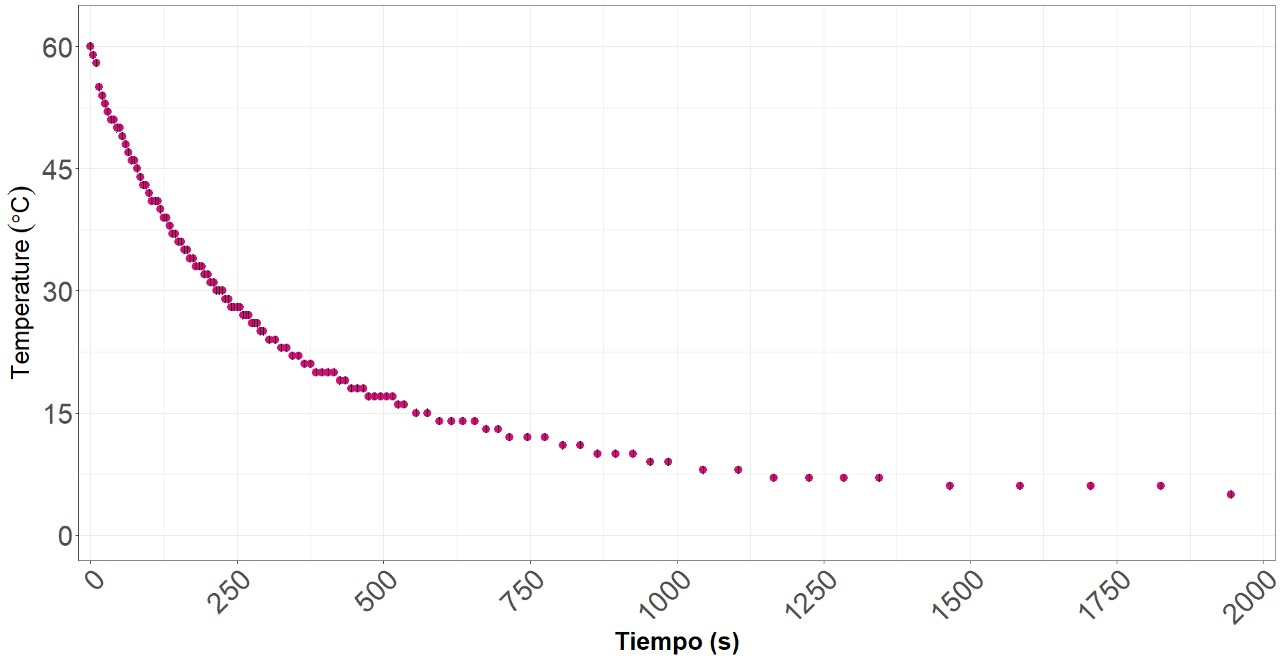
\includegraphics[width=0.8\linewidth]{60cal.png}
    \caption{Gráfica de la disminución de temperatura desde 60°C}
    \label{fig:enter-label}
\end{figure}
\begin{multicols}{2}
    
Mismo caso para los 60°C la diferencia de temperatura que causa el hielo cambia los resultados experimentales.\\
Cuando hay una gran diferencia de temperatura entre dos ambientes, uno muy frío y otro a temperatura ambiente, ocurren varios fenómenos físicos que afectan el intercambio de calor y la interacción entre estos ambientes. 
Conducción: Si hay algún contacto físico entre los dos ambientes (aunque sea indirecto a través de un material conductor), el calor se transferirá rápidamente del ambiente más cálido al más frío. En este caso, el ambiente frío absorberá calor del ambiente más cálido.

Convección: En un entorno con aire o fluido, la diferencia de temperatura genera corrientes de convección. El aire caliente se elevará y el aire frío descenderá, creando ciclos de flujo de aire que ayudan a igualar las temperaturas. \\
\textbf{Observación:}Esto tambien es algo a notar, pues durante el experimento justo al momento de sacar el agua del fuego se producía un breve aumento de temperatura a pesar de ya no recibir calor, esto puede deberse al movimiento del agua mas caliente y el agua mas fria a través del vaso por convección

Radiación: La transferencia de calor también puede ocurrir a través de la radiación térmica. Los cuerpos emiten radiación infrarroja, y el cuerpo más cálido emitirá más radiación, la cual será absorbida por el cuerpo más frío.

\section{Conclusiones y recomendaciones}
Podemos concluir que La Ley de Enfriamiento de Newton establece que la tasa de cambio de la temperatura de un objeto es proporcional a la diferencia entre la temperatura del objeto y la temperatura del entorno. Se expresa mediante la ecuación (1), con su solución (6).
\textbf{Tasa de Enfriamiento:} La tasa a la cual el objeto se enfría (o calienta) es directamente proporcional a la diferencia de temperatura entre el objeto y el entorno. Cuanto mayor es esta diferencia, mayor es la tasa de cambio de temperatura.

\textbf{Ecuación de Enfriamiento:} La solución a la ecuación diferencial, asumiendo que la temperatura del objeto en el tiempo $t=0$ es $T_0$ es la ecuación (5).

\textbf{Dependencia del Coeficiente de Enfriamiento: } La constante $k$ refleja las propiedades del objeto, como su capacidad calorífica y la tasa de transferencia de calor. Un valor mayor de $k$ indica un enfriamiento más rápido debido a una mayor transferencia de calor.

 La Ley de Enfriamiento de Newton proporciona una descripción matemática precisa de cómo un objeto pierde calor en un entorno de temperatura constante. La tasa de enfriamiento es proporcional a la diferencia de temperatura entre el objeto y el entorno, lo que resulta en un enfriamiento exponencial. Esta ley es fundamental para entender y predecir el comportamiento térmico en una amplia gama de aplicaciones científicas y técnicas. Su capacidad para modelar la dinámica del enfriamiento y calentamiento facilita la resolucion de problemas.
\end{multicols} 

\section{Apéndice}

\begin{figure}[H]
    \centering
    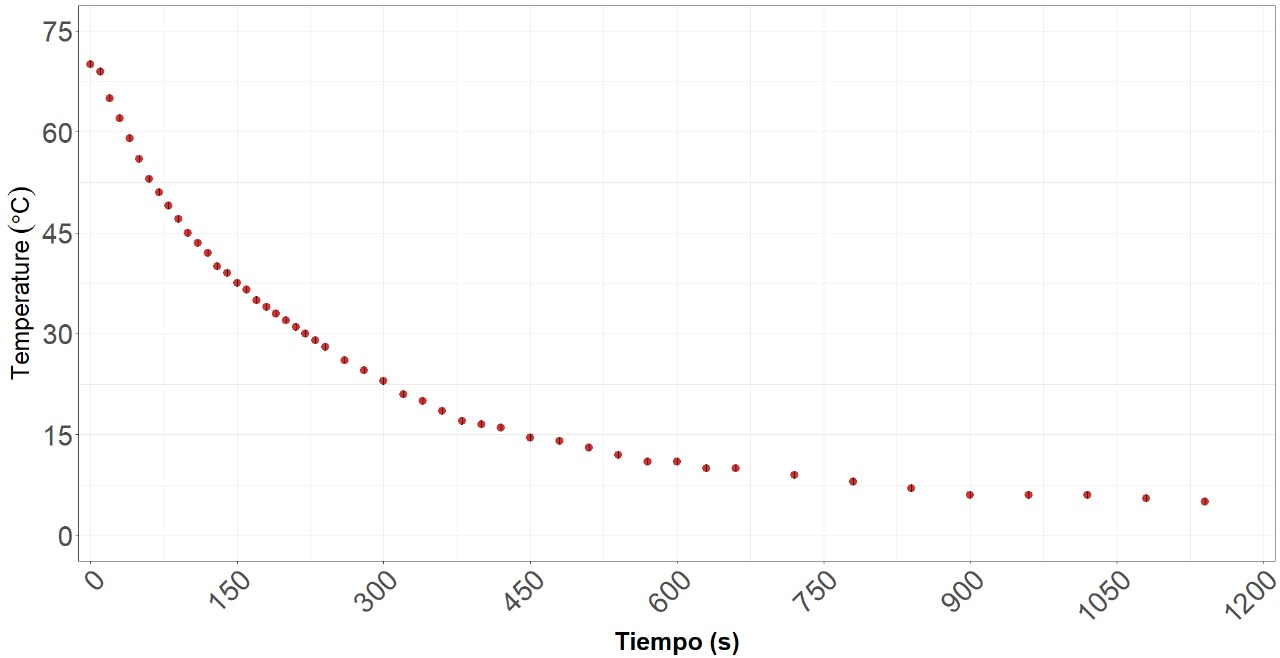
\includegraphics[width=0.9\linewidth]{70cal.png}
    \caption{Mediciones de la temperatura con respecto a in-
tervalos de tiempo 70°C. $\pm$ 0.5C}
    \label{fig:enter-label}
\end{figure}

\begin{figure}[H]
    \centering
    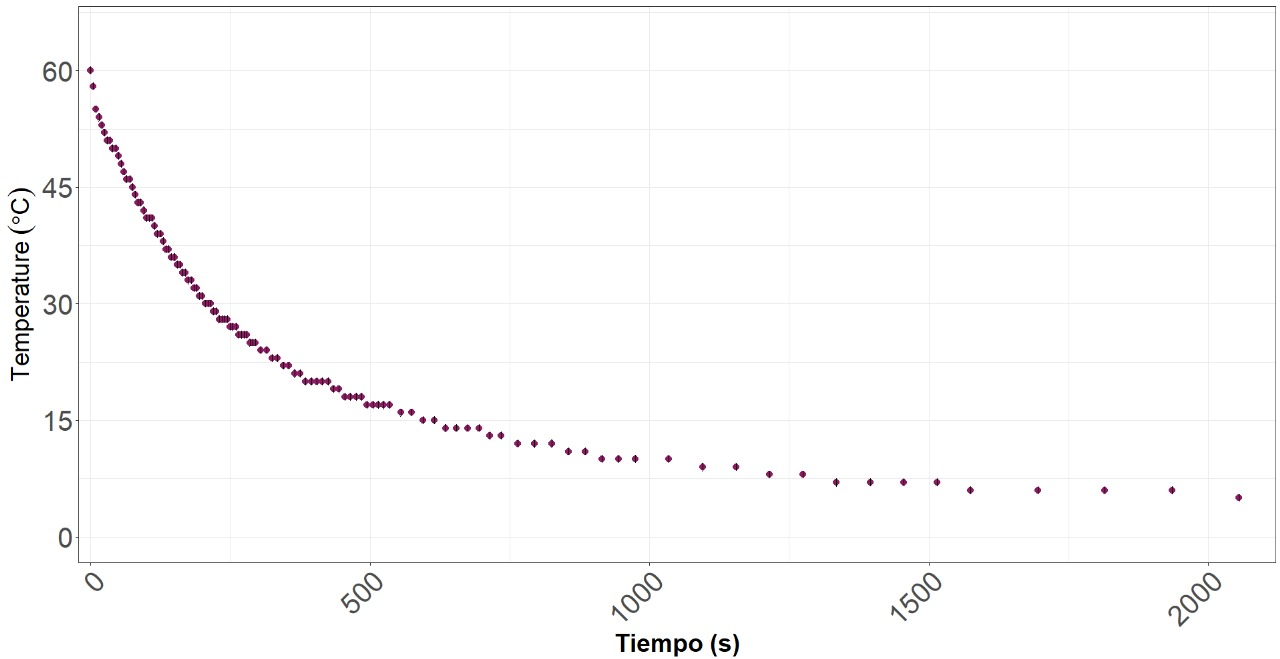
\includegraphics[width=0.9\linewidth]{80cal.png}
    \caption{Mediciones de la temperatura con respecto a in-
tervalos de tiempo 80°C. $\pm$ 0.5C}
    \label{fig:enter-label}
\end{figure}

\newpage
\begin{multicols}{2}
    

\begin{tabular}{|c|c|}
		\hline
		\textbf{Tiempo (s)} & \textbf{Temperatura (°C)} \\ \hline
		0    & 80.0  \\ \hline
		10   & 79.0  \\ \hline
		20   & 77.0  \\ \hline
		30   & 74.0  \\ \hline
		40   & 71.0  \\ \hline
		50   & 69.0  \\ \hline
		60   & 65.0  \\ \hline
		70   & 62.0  \\ \hline
		80   & 59.0  \\ \hline
		90   & 56.5  \\ \hline
		100  & 54.0  \\ \hline
		110  & 52.0  \\ \hline
		120  & 49.5  \\ \hline
		130  & 47.5  \\ \hline
		140  & 45.5  \\ \hline
		150  & 44.0  \\ \hline
		160  & 42.0  \\ \hline
		170  & 40.5  \\ \hline
		180  & 39.0  \\ \hline
		190  & 38.0  \\ \hline
		200  & 36.5  \\ \hline
		210  & 35.0  \\ \hline
		220  & 34.0  \\ \hline
		230  & 33.0  \\ \hline
		240  & 32.0  \\ \hline
		260  & 30.5  \\ \hline
		280  & 29.0  \\ \hline
		300  & 27.0  \\ \hline
		320  & 26.0  \\ \hline
		340  & 25.0  \\ \hline
		360  & 24.0  \\ \hline
		380  & 22.5  \\ \hline
		400  & 21.5  \\ \hline
		420  & 21.0  \\ \hline
		450  & 19.5  \\ \hline
		480  & 18.5  \\ \hline
		510  & 17.0  \\ \hline
		540  & 16.5  \\ \hline
		570  & 16.0  \\ \hline
		600  & 15.0  \\ \hline
		630  & 14.0  \\ \hline
		660  & 14.0  \\ \hline
		720  & 13.0  \\ \hline
		780  & 12.0  \\ \hline
		840  & 11.0  \\ \hline
		900  & 10.0  \\ \hline
		1020 & 9.0   \\ \hline
		1080 & 8.0   \\ \hline
		1260 & 7.0   \\ \hline
		1380 & 6.0   \\ \hline
		1620 & 5.0   \\ \hline
	\end{tabular}

	\begin{tabular}{|c|c|}
		\hline
		\textbf{Tiempo (s)} & \textbf{Temperatura (°C)} \\ \hline
		0    & 70.0 \\ \hline
		10   & 69.0 \\ \hline
		20   & 65.0 \\ \hline
		30   & 62.0 \\ \hline
		40   & 59.0 \\ \hline
		50   & 56.0 \\ \hline
		60   & 53.0 \\ \hline
		70   & 51.0 \\ \hline
		80   & 49.0 \\ \hline
		90   & 47.0 \\ \hline
		100  & 45.0 \\ \hline
		120  & 42.0 \\ \hline
		140  & 39.0 \\ \hline
		160  & 36.5 \\ \hline
		180  & 34.0 \\ \hline
		200  & 32.0 \\ \hline
		210  & 31.0 \\ \hline
		220  & 30.0 \\ \hline
		230  & 29.0 \\ \hline
		240  & 28.0 \\ \hline
		260  & 26.0 \\ \hline
		280  & 24.5 \\ \hline
		300  & 23.0 \\ \hline
		320  & 21.0 \\ \hline
		340  & 20.0 \\ \hline
		360  & 18.5 \\ \hline
		380  & 17.0 \\ \hline
		400  & 16.5 \\ \hline
		420  & 16.0 \\ \hline
		450  & 14.5 \\ \hline
		480  & 14.0 \\ \hline
		510  & 13.0 \\ \hline
		540  & 12.0 \\ \hline
		570  & 11.0 \\ \hline
		600  & 11.0 \\ \hline
		630  & 10.0 \\ \hline
		660  & 10.0 \\ \hline
		720  & 9.0  \\ \hline
		780  & 8.0  \\ \hline
		840  & 7.0  \\ \hline
		900  & 6.0  \\ \hline
		960  & 6.0  \\ \hline
		1020 & 6.0  \\ \hline
		1080 & 5.5  \\ \hline
		1140 & 5.0  \\ \hline
	\end{tabular}


\end{multicols}
\newpage

\begin{multicols}{2}

Las tablas pertenecen respectivamente a Mediciones de la temperatura con respecto a in-
tervalos de tiempo 80°C. $\pm$ 0.5C con calorimetro y Mediciones de la temperatura con respecto a intervalos de tiempo 70°C. $\pm$ 0.5C

Ahora veamos el ajuste por mínimos cuadrados.\\
De la ecuación
\begin{equation}
    (T(t)-T_A) = e^{kt+C} \rightarrow \ln((T(t)-T_A) = kt+C
\end{equation}

Se calcula con los mínimos cuadrados
\begin{equation}
    k = \frac{\Sigma xy-(\Sigma x)(\Sigma y)}{n \Sigma x^2 -(\Sigma x)^2}
\end{equation}

Donde\\
x: tiempo\\y: $\ln(T(t)-T_A)$\\n: cantidad de calor

$b = x - k\overline{x}$ $k\overline{x} = $ Promedio de $\ln(T(t)-T_A)$\\
$c = y - k\overline{y}$ $k\overline{x} = $ Promedio de tiempo.

\textbf{60°C Sin calorímetro}
\begin{equation}
    k = \frac{18(251460 - (5130)(924)}{18(1898100)-(26316900)}
\end{equation}
Donde \\
$\Sigma xy = 251460$\\ 
$\Sigma x = 5130$ \\
$\Sigma y = 924$ \\
$\Sigma x^2 = 1898100 \\
n = 100

\begin{equation}
    k = \frac{4526280 - 4740120}{3565800- 26316900}
\end{equation}

\begin{equation}
    k = \frac{213840}{-22751100} = 9.39 \times 10^{-3}
\end{equation}

\textbf{80°C sin calorímetro}

\begin{equation}
    k = \frac{22(701610 - (12630)(1331)}{22(12852900) - (1771061)}
\end{equation}

Donde \\
$\Sigma xy = 701610$\\ 
$\Sigma x = 12630$ \\
$\Sigma y = 1331$ \\
$\Sigma x^2 = 12852900 \\
n = 22

\begin{equation}
    k = \frac{-1375110}{280992739} = -0.0489
\end{equation}

\textbf{60°C con calorímetro}

\begin{equation}
    k = \frac{112(733125) - 1129680(3003)}{112(37434050) - 1.27 \times 10^{-12}}
\end{equation}

Donde \\
$\Sigma xy = 733121$\\ 
$\Sigma x = 1128680$ \\
$\Sigma y = 3003$ \\
$\Sigma x^2 = 37434080$ \\
$(\Sigma x)^2 = 1.27 \times 10^{-12}$ \\
n = 112

\begin{equation}
    k = \frac{-3310319040}{-1.2658 \times 10^{-12}} = 2.8395 \times 10^{21}
\end{equation}

\textbf{80°C con calorímetro}
\begin{equation}
    k = \frac{122(1025330 - (53990)(4112)}{122(42271300) - (2914920100)}
\end{equation}

Donde \\
$\Sigma xy = 1025330$\\ 
$\Sigma x = 53990$ \\
$\Sigma y = 4112$ \\
$\Sigma x^2 = 42271300$ \\
$(\Sigma x)^2 = 2914920100$ \\
n = 112

\begin{equation}
    k = \frac{-96916620}{224217880} = -0.04222
\end{equation}

\end{multicols}

\bibliography{biblio}
    [1] Sears, F. W., Zemansky, M. W., & Young, H. D. (2012). Física universitaria con física moderna (13ª ed., Vol. 1). Pearson Educación.

    [2] Halliday, D., Resnick, R., & Walker, J. (2010). Fundamentals of Physics (9th ed.). Wiley.

[3 [Leskow, E. C. (s/f-a). Temperatura - Concepto, tipos, escalas y medición, de https://concepto.de/temperatura/

[4] Leskow, E. C. (s/f-b). Termodinámica - Concepto, leyes y sistema termodinámico, de https://concepto.de/termodinamica/
    

    
    [5] Zemansky, M. W., & Dittman, R. H. (1997). Heat and Thermodynamics (7th ed.). McGraw-Hill.
    
\end{document}